\newpage

\section{Measuring Voltage Across a Potentiometer}
\label{s:voltage}

\subsection{Parts List}

\begin{enumerate}[itemsep=-5pt]
\item Laptop
\item CPX/CPB
\item USB Cable
\item Potentiometer
\item Resistor (the Ohms depends on how large your potentiometer is)
\item Breadboard
\end{enumerate}

\subsection{Learning Objectives}
\begin{enumerate}[itemsep=-5pt]
\item Understand voltage division of resistors in series
\item Measure an analog signal on the CircuitPlayground
\item Understand the binary measurement done by the analog to digital conversion (ADC)
\end{enumerate}

\subsection{Getting Started}

At this point you've learned about analog to digital converters (ADC). It turns out that the CPX has 8 analog ports hooked up to a 3.3V logic 16 bit ADC. The input range on the ADC is 0 to 3.3V and the output range is 0 to 65536 which is $2^{16}$ hence 16 bits. In order to get accustomed to the ADC on the CPX, we’re going to do a simple example where we measure the voltage drop across a potentiometer. You can read about \href{https://www.build-electronic-circuits.com/potentiometer/}{potentiometers online if you wish}. Basically though, a potentiometer is a variable resistance resistor that changes resistance by turning a knob. The knob changes the connection point of a wire and thus the length of the wire. This in turn changes the resistance. Potentiometers come in all shapes and sizes. Here are some \href{https://uk.rs-online.com/web/content/discovery/ideas-and-advice/potentiometers-guide}{potentiometer examples}. I've done this lab with a few potentiometer. Ideally you'd like to have the potentiometer hooked up in serie with another resistor so that you end up building a voltage divider but it' possible you can do it without it. Here’s my circuit all hooked up without a resistor in series. Two legs are connected to 3.3V and GND while the middle leg of the potentiometer is connected to pin A2.
\begin{figure}[H]
  \begin{center}
    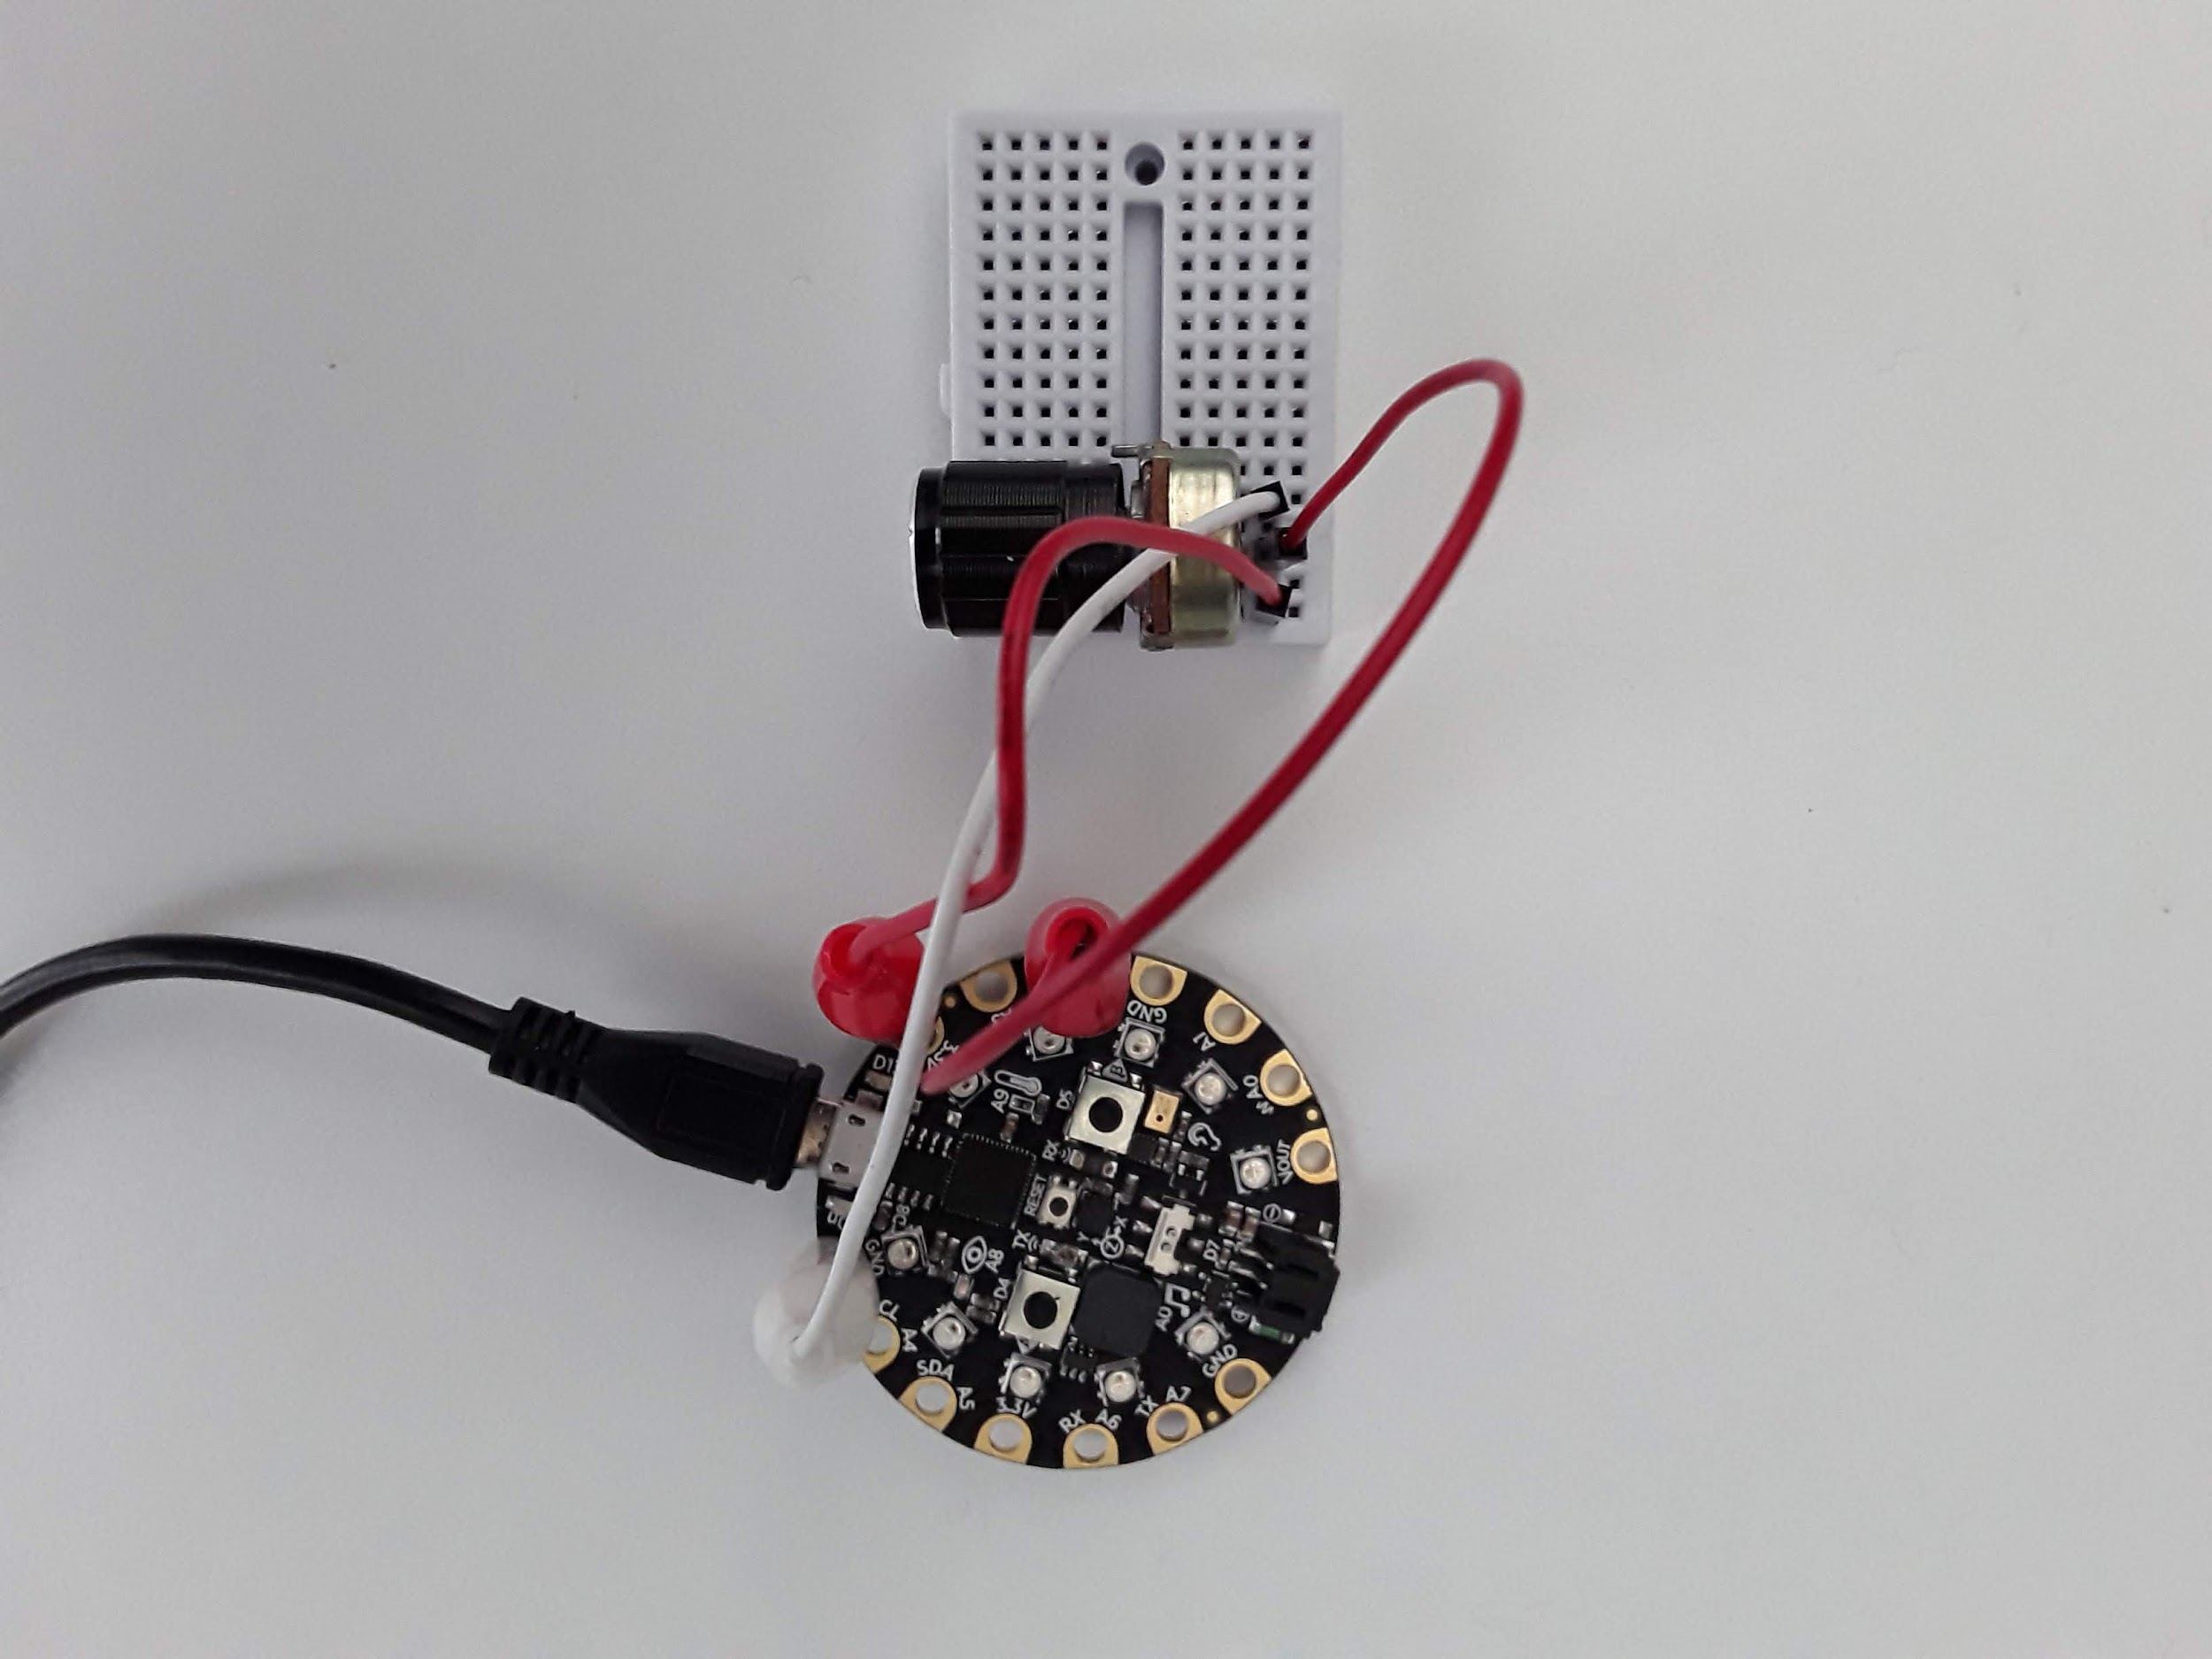
\includegraphics[width=0.8\textwidth]{Figures/potentiometer1.jpeg}
  \end{center}
\end{figure}
{\bf As I said before, some potentiometers do not have enough resistance when turned all the way down. I suggest that you put a resistor in between the third leg and ground. Some experimenters have melted plastic or gotten really hot. One student even blew up a potentiometer.} Here is my circuit with a resistor in series.
\begin{figure}[H]
  \begin{center}
    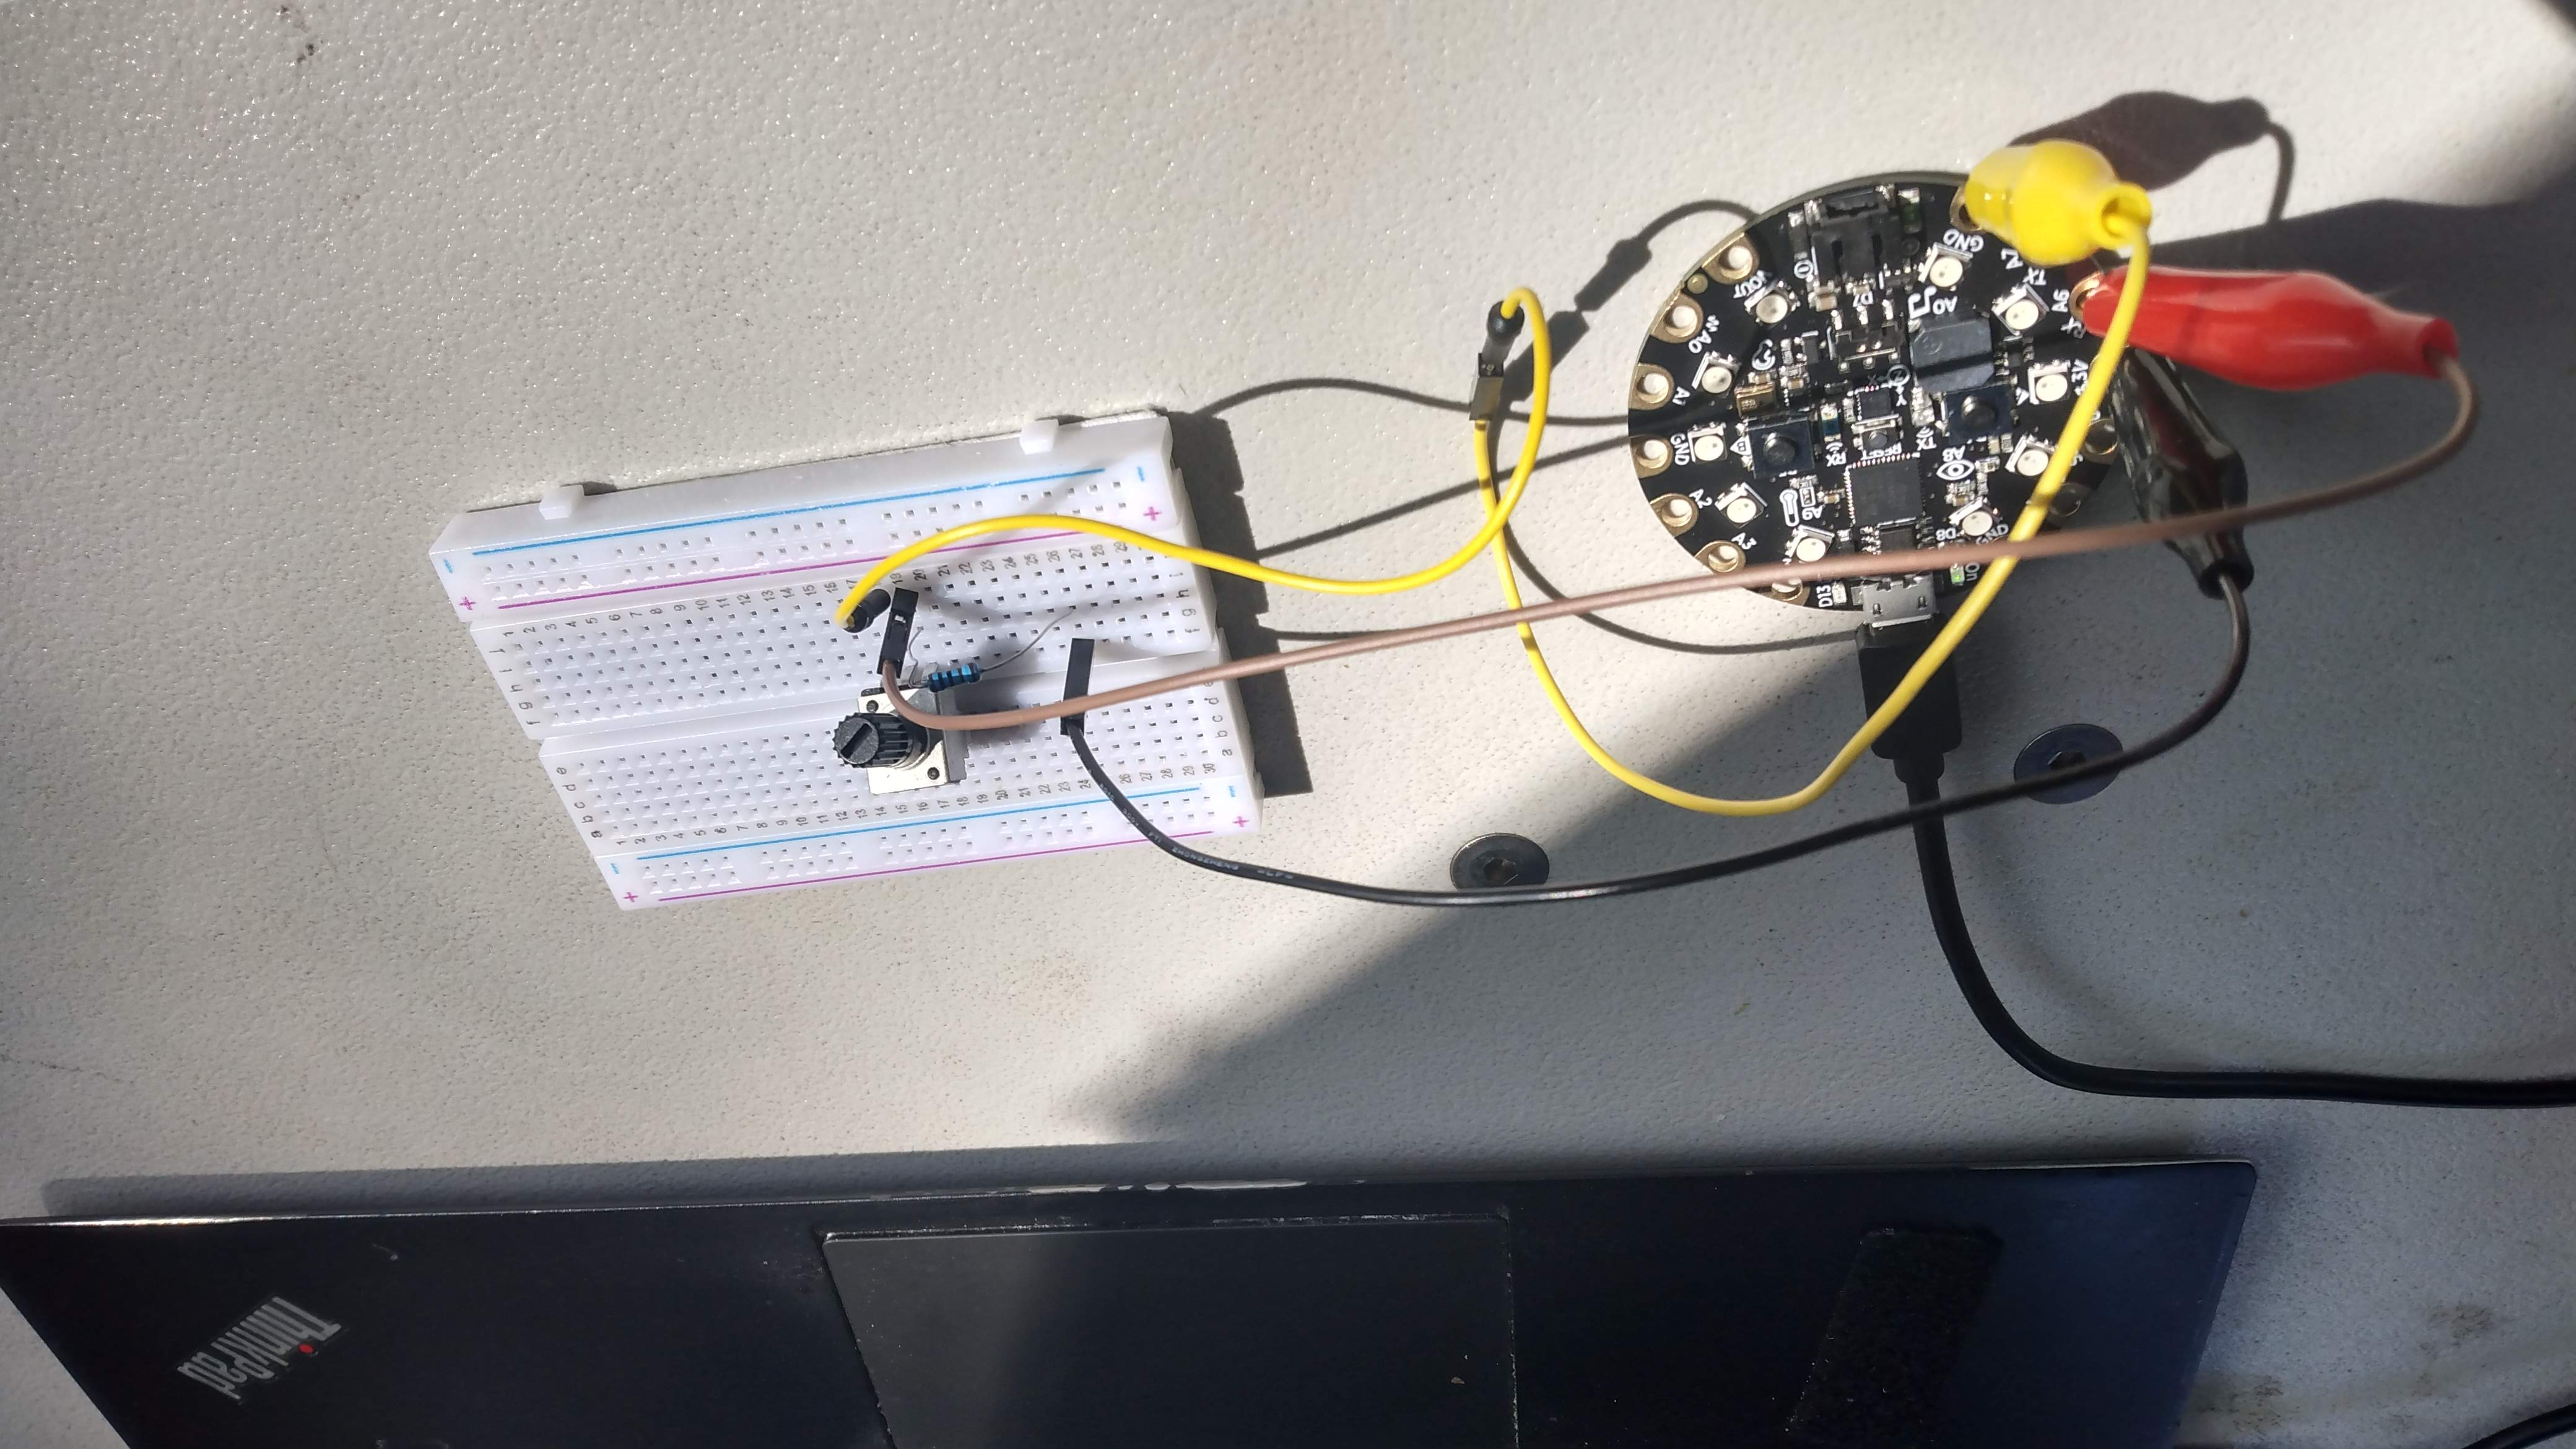
\includegraphics[angle=180,width=0.8\textwidth]{Figures/Potentiometer_Alternate.jpg}
  \end{center}
\end{figure}
There is a relevant \href{https://learn.adafruit.com/adafruit-circuit-playground-express/circuitpython-analog-in}{Adafruit Learn Tutorial} to help with the {\it analogio} module but I’ll explain the minimum required here to get some analog values plotted in {\it Plotter} and Python on your computer. First let’s take a look at some \href{https://github.com/cmontalvo251/Microcontrollers/blob/master/Circuit_Playground/CircuitPython/Analog/analog_simple.py}{simple example code} to read an analog signal and plot it using the {\it Plotter}.
\begin{figure}[H]
  \begin{center}
    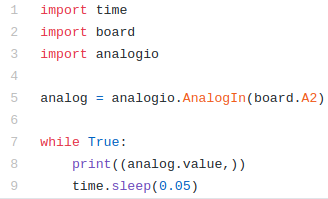
\includegraphics[width=0.5\textwidth]{Figures/analogio.png}
  \end{center}
\end{figure}
In the example code above, lines 1-3 again import the necessary modules with {\it analogio} being the new module here. Line 5 creates the analog object by attaching pin A2 to the analog function. Lines 7-9 then simple read the analog value and print it to {\it Serial} and the {\it Plotter}. Running this code on my laptop and turning the knob on the potentiometer produces this output. My potentiometer has a very large knob on the front and is easy to turn. Some potentiometers have a small screw on top that you need to turn with a screwdriver. Turning the screw or the knob results in chaning the resistance and therefore changing the voltage read by the CPX.
\begin{figure}[H]
  \begin{center}
    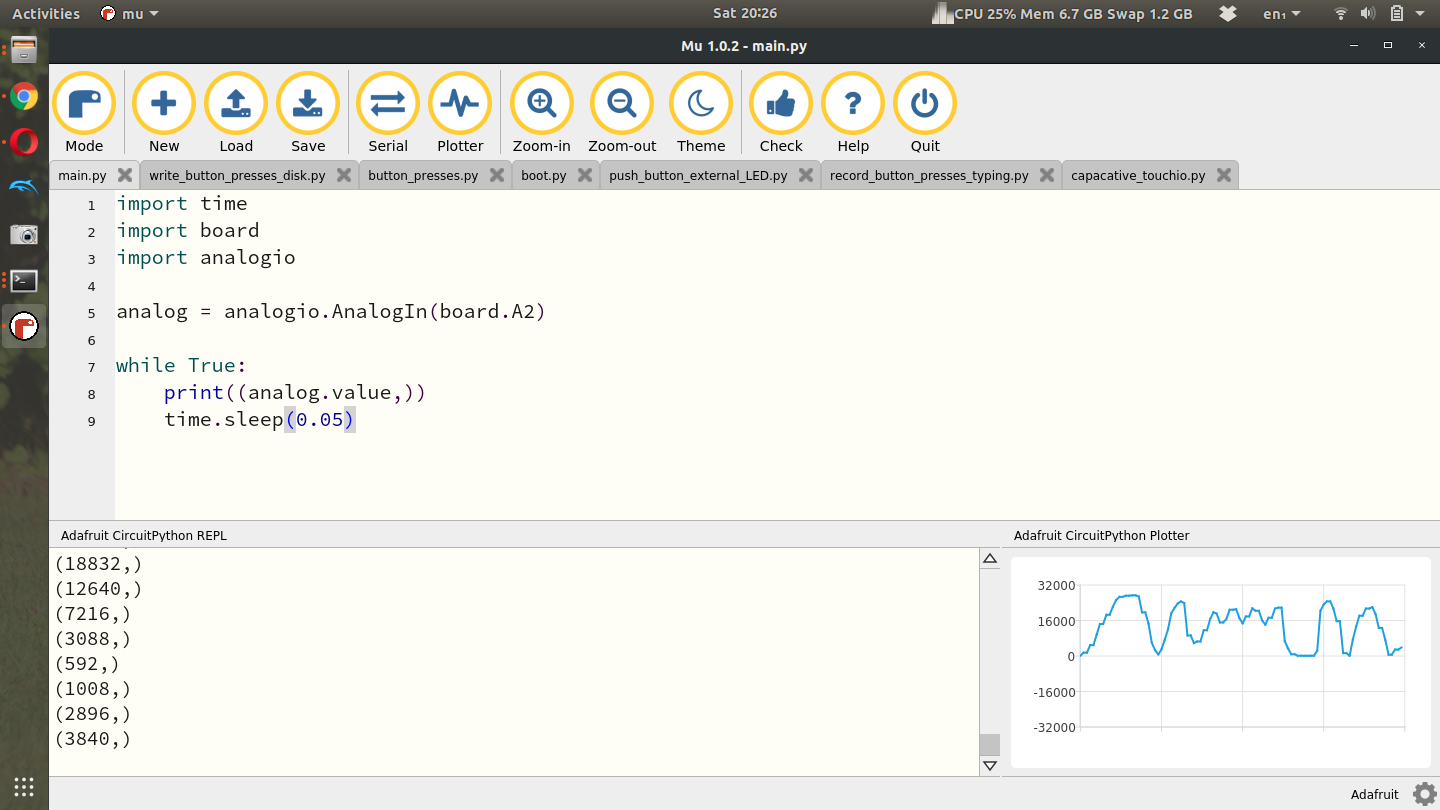
\includegraphics[width=\textwidth]{Figures/analogio_mu.png}
  \end{center}
\end{figure}
For this lab I want you to spin the potentiometer all the way to one side and then the other while recording time and the analog value. I then want you to plot the data with time on the x-axis and voltage on the y-axis. Remember to convert a digital output to voltage you just need to use the equation below where D is the raw value from the analog port. 3.3V is the range of the ADC and $2^{16}$ is the maximum value the ADC can represent.
\begin{equation}
V = \frac{3.3D}{2^{16}}
\end{equation}
After doing this experiment myself, this is the plot I obtain. The code is not provided as reading data and plotting has been discussed in a previous lab (See chapter \ref{s:daq}). From the screenshot though you can see how I convert the digital output to an analog signal.
\ \\
\ \\
{\bf NOTE THAT ON LINE 6 IT READS}
\begin{verbatim}
time -= time[0]
\end{verbatim}
{\bf Notice the minus sign in front of the equal sign. That effects a lot.}
\begin{figure}[H]
  \begin{center}
    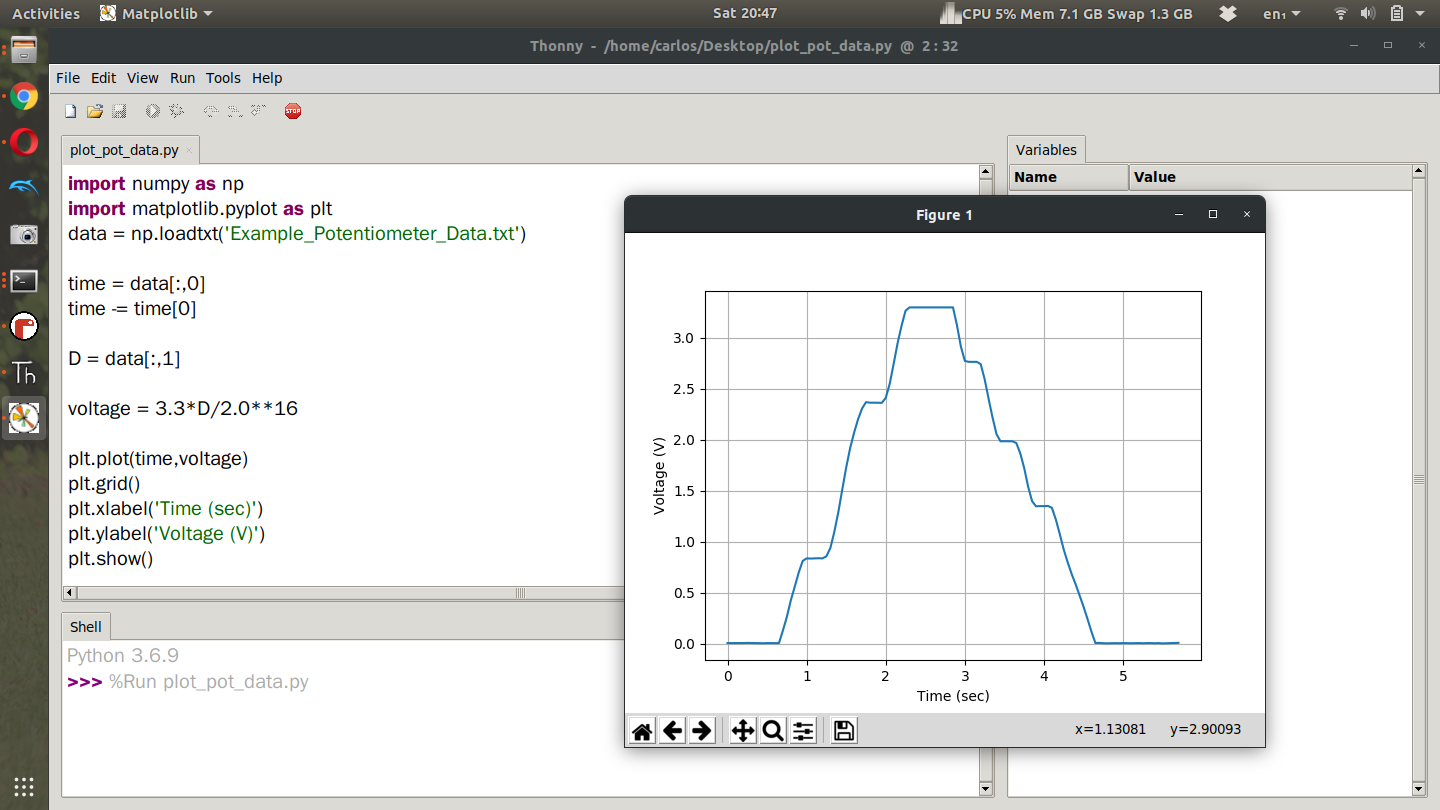
\includegraphics[width=\textwidth]{Figures/plotting_analogio.png}
  \end{center}
\end{figure}
Your assignment for this lab is to do the same as I’ve done above. Wire up the potentiometer, read the analog signal and plot it in Python on your desktop computer. I’ve made some youtube videos on first just \href{https://youtu.be/_gnDvPOvPqk}{creating the circuit and plotting the data} and then another video where I \href{https://youtu.be/9UF3OVUIYjU}{write data to the CPX using method 3}.

\subsection{Assignment}

Once you've completed the project above, upload a PDF with all of the photos and text
below included. My recommendation is for you to create a Word document
and insert all the photos and text into the document. Then export the
Word document to a PDF. For videos I suggest uploading the videos to
Google Drive, turn on link sharing and include a link in your
PDF. {\bf Note that all code must be included in the appendix or you'll be
penalized 10\%.}
\ \\

{\bf For all videos you must explain what you're doing. At a minimum state your name and explain what your circuit does.}


\begin{enumerate}[itemsep=-5pt]
\item Include a video of you showing your circuit and then rotate the potentiometer back and forth and watch the digital signal in the Plotter in Mu go up and down - 50\%
\item Plot your digital output (raw potentiometer analog value) vs time - 25\%
\item Then convert your digital output (Do) to voltage and plot that vs time - 25\% 
\end{enumerate}
